\section{(key, value) Vector}

\subsection{Key}
\begin{frame}
    \frametitle{Key}
	\begin{itemize}
		\item Key indicate neural id.
    	\begin{figure}
			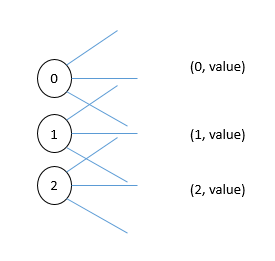
\includegraphics[scale=0.5]{figure/key.png}
		\end{figure}
	\end{itemize}
\end{frame}

\subsection{Value}
\begin{frame}
    \frametitle{Value}
	\begin{itemize}
		\item Value indicate weights with respect to the neural id. 
    	\begin{figure}
			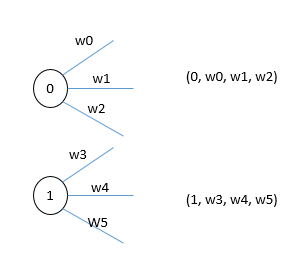
\includegraphics[scale=0.5]{figure/value.png}
		\end{figure}
	\end{itemize}
\end{frame}

\subsection{Vector}
\begin{frame}
    \frametitle{Vector}
	\begin{itemize}
		\item Vector is the combination of key and values.
		\item Vector is the minimum communication unit.
	\end{itemize}
\end{frame}


